\documentclass[11pt,a4paper]{article}

\usepackage{main}
\usepackage{cours}

\renewcommand{\typedocument}{Cours}
\renewcommand{\classe}{3e}
\renewcommand{\titre}{Energie}

\begin{document}

\pagination

\creertitre{L'Énergie}

\partie{Les formes  d'énergie}

L'\important{énergie} est une \textbf{grandeur physique} qui correspond à la capacité d'un système à agir en fournissant un travail.

Son \textbf{unité} principale est le \important{Joule (J)} mais il existe aussi d'autres unités pour l'énergie comme le wattheure (1 Wh = 3600 J) ou la calorie (1 cal = 4,18 J).

L'énergie peut se présenter sous 6 formes différentes :
\begin{itemize}
    \item \important{L'énergie mécanique}, liée au mouvement et à l'altitude des objets, \item[] \exemple{L'énergie d'une voiture en mouvement}
    \item \important{L'énergie électrique}, qui circule dans les circuits électriques,
    \item[] \exemple{L'énergie utilisé par un ordinateur ou un four}
    \item \important{L'énergie lumineuse}, comme celle qui provient du Soleil pour nous éclairer,
    \item[] \exemple{L'énergie produite par une lampe LED}
    \item \important{L'énergie thermique}, qui correspond à la chaleur
    \item[] \exemple{L'énergie produite par un radiateur},
    \item \important{L'énergie chimique}, contenue dans ce qui peut faire des réactions chimiques,
    \item[] \exemple{L'énergie utilisée par le corps humain, ou contenue dans une pile}
    \item \important{L'énergie nucléaire}, contenue dans ce qui peut faire des réactions nucléaires.
    \item[] \exemple{l'énergie contenue dans l'Uranium}
\end{itemize}

\partie{Transferts et conversions d'énergie}

\souspartie{Définitions}

Un système peut donner à un autre système une forme d'énergie, on parle de \important{transfert d’énergie}.\\
\exemple{En posant une casserole sur le feu, l'énergie thermique est transférée du feu à la casserole, puis de la casserole à son contenu.}

Un système peut convertir une forme d'énergie en une autre, on parle de \important{conversion d'énergie}.\\
\exemple{Une éolienne convertit l'énergie mécanique du vent en énergie électrique.}

\souspartie{Bilan énergétique et chaîne énergétique}

L'énergie ne peut être ni créée, ni détruite. C'est le \important{principe de conservation de l'énergie}. Elle peut être transférée d’un objet à un autre ou convertie d’une forme en une autre.

On peut représenter ces changements avec des \important{schémas de chaîne énergétique} :

\begin{center}
    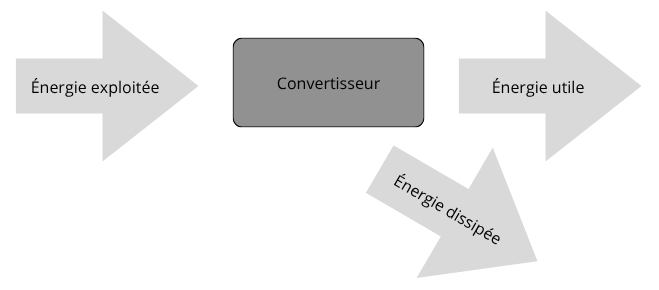
\includegraphics[width=10cm]{images/chaine énergétique exemple.png}
\end{center}

\newpage

Une partie de l'\important{énergie exploitée} est convertie en énergie exploitable (\important{énergie utile}), et le reste de l'énergie est souvent perdu (\important{énergie dissipée}) : $E_{exploit\acute e e} = E_{utile} + E_{dissip\acute  ee}$.

\exemple{On étudie le système dynamo+lampe d'un vélo. La dynamo convertit l'énergie mécanique des roues en énergie électrique, qui est transmise à la lampe. Ensuite, la lampe convertit l'énergie électrique en énergie lumineuse. A chaque étape, de l'énergie est perdue sous forme de chaleur.}

\begin{center}
    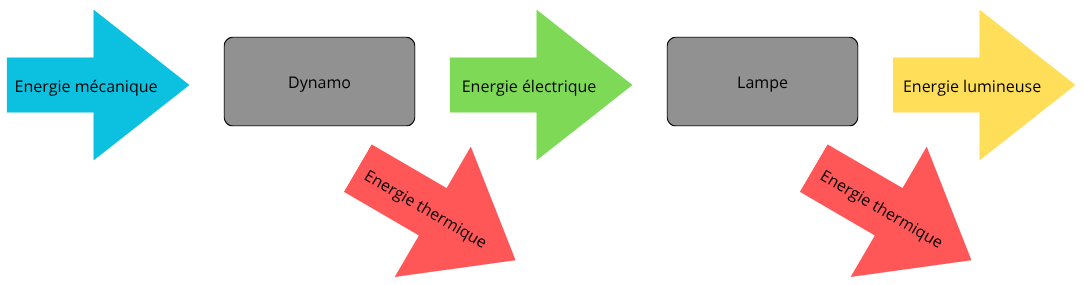
\includegraphics[width=14cm]{images/chaine énergétique dynamo-lampe.png}
\end{center}

\partie{L'énergie mécanique}

L'\important{énergie mécanique} d'un objet est composée de son \important{énergie cinétique}, liée à la vitesse de l'objet, et de son \important{énergie potentielle de pesanteur}, liée à la position de l'objet.

\textbf{L'énergie cinétique} $E_c$ d'un objet augmente lorsque sa masse $m$ ou sa vitesse $v$ augmente.

\begin{center}
    \LARGE\important{$E_c = \frac{1}{2} \times m \times v^2$}
\end{center}

où :
\begin{itemize}
    \item $E_c$ est l'\textbf{énergie cinétique de l'objet en joules (J)},
    \item $m$ est la \textbf{masse de l'objet en kilogrammes (kg)},
    \item $v$ est la \textbf{vitesse de l'objet en mètres par seconde (m/s)}.
\end{itemize}

\vspace{6pt}

\exemple{On considère une voiture de masse $m = \SI{1000}{\kilogram}$ lancée à 30 m/s.\\
Son énergie cinétique vaut : $E_c = \frac{1}{2} \times m \times v^2 = \frac{1}{2} \times 1000 \times 30^2 = \SI{450000}{\joule}$.}

\textbf{L'énergie potentielle de pesanteur} est due à l'interaction de gravitation entre la Terre et l'objet. L'énergie potentielle de pesanteur $E_p$ diminue lorsque l'altitude $h$ de l'objet diminue.

\begin{center}
    \LARGE\important{$E_p = m \times g \times h$}
\end{center}

où :
\begin{itemize}
    \item $E_p$ est l'\textbf{énergie potentielle de pesanteur de l'objet en joules (J)},
    \item $m$ est la \textbf{masse de l'objet en kilogrammes (kg)},
    \item $g$ est l'\textbf{intensité de la pesanteur (9,8 N/kg sur Terre)},
    \item $h$ est la \textbf{hauteur de l'objet en mètres (m)}.
\end{itemize}

\vspace{6pt}

\exemple{On considère une pomme de masse $m = \SI{100}{\gram}$ dans un arbre à une distance $h=\SI{2}{\meter}$ du sol.\\
Son énergie potentielle de pesanteur vaut : $E_p = m \times g \times h = 0,1 \times 9,8 \times 2 = \SI{1,96}{\joule}$.}

\newpage

L'énergie mécanique $E_m$ est la somme de l'énergie cinétique $E_c$ et de l'énergie potentielle de pesanteur $E_p$ : \important{$E_m = E_c + E_p$}.

Lors de la \textbf{chute} d’un corps, l’énergie potentielle de position diminue et se convertit en énergie cinétique (qui augmente). L’énergie mécanique \textbf{se conserve} s’il n’y a pas de pertes à cause des frottements.

\exemple{Si on garde l'exemple de la pomme, au moment où elle se détache de l'arbre elle a une énergie cinétique nulle, qui va augmenter au faire et à mesure qu'elle tombera, alors que son énergie potentielle diminuera.}


\partie{Puissance d'un appareil}

La puissance $P$ correspond à l'énergie échangée par un système $E$ pendant une durée $t$. Elle s'exprime en \important{Watt (W)}.

Le terme de puissance est souvent utilisé pour qualifier des appareils électriques. Plus l’appareil est puissant, plus l’énergie consommée sera grande.
Plus le temps de fonctionnement sera important, plus l’énergie consommée sera grande.

\begin{center}
    \LARGE\important{$P = E \div t$} ou \LARGE\important{$E = P \times t$}
\end{center}

où :
\begin{itemize}
    \item $E$ est l'\textbf{énergie en joules (J)},
    \item $P$ est la \textbf{puissance en Watt (W)},
    \item $t$ est la \textbf{durée en secondes (s)}.
\end{itemize}

\vspace{6pt}

On utilise parfois un autre système d'unités : si le temps est donné en \important{heures (h)}, alors l'énergie sera en \important{wattheures (Wh)}. Ce sont ces unités que l'on retrouve sur les factures d'électricité par exemple.

\exemple{J'utilise mon ordinateur 5 heures dans la journée, il consomme 450 W.\\
$E = P \times t = 450 \times 5 = \SI{2250}{\watt \hour}$\\
$E = P \times t = 450 \times 5 \times 3600 = 8,1 \times 10^{6} \SI{}{\joule}$\\
La dépense énergétique journalière de l'ordinateur est de 2250 Wh ou $8,1 \times 10^{6} \SI{}{\joule}$. On peut garder la durée en heures pour obtenir des wattheures, ou convertir en secondes pour un résultat en joules. $\SI{1}{\watt \hour} = \SI{3600}{\joule}.$
}

\partie{Les sources d'énergie}

Les activités humaines consomment de l'énergie. Pour se développer, les êtres humains reposent donc sur des \important{sources d'énergie primaires}.

Certaines sources d'énergie sont \important{renouvelables}, c'est-à-dire qu'elles sont inépuisables à l’échelle de l’humanité.
\exemple{Le soleil, l'eau, le vent.}

D'autres sources d'énergie sont \important{non-renouvelables}, leurs stocks sur Terre
sont limités ou se renouvellent trop lentement. Il y a :
\begin{itemize}
    \item Les \important{sources fossiles}. Ces substances ont mis des millions d'années à se former et leur combustion produit d'énormes quantités de gaz à effet de serre.
    \item[] \exemple{Gaz naturel, charbon, pétrole}
    \item Les \important{sources nucléaires}. Cette ressource d'énergie produit des déchets nucléaires mais n'émet pas directement de gaz à effet de serre.
    \item[] \exemple{L'uranium} 
\end{itemize}

Dans le cadre du développement durable, les humains doivent réduire leur consommation d'énergie et privilégier les sources d'énergie renouvelables.

\end{document}